\FloatBarrier
\subsection{Completed language and label-shift comparisons}\label{app:language-shift-complete}
\paragraph{Language protocol and endpoint.} All ten WikiText-103/GPT-2-small candidates finish their declared budget before selection. The model has 123849984 parameters and trains from scratch; projected methods use maximum rank 16. Each run uses 1000 units of ten updates, batch size eight and context length 256, totaling 10000 updates and 20480000 training tokens. These are fixed-token-budget comparisons, not 1000-corpus-epoch runs. Each method independently selects between $3\times10^{-4}$ and $10^{-3}$ using mean validation cross-entropy over units 901--1000. Reported perplexity is $\exp(100^{-1}\sum_{u=901}^{1000}\ell_u)$, not the arithmetic mean of per-unit perplexities; the same selected configuration supplies its test endpoint. All candidates use seed 42 and identical frozen token splits. Complete candidate endpoints remain in Appendix~\ref{app:new-completions}.

\begin{table}[htbp]\centering\footnotesize
\caption{\textbf{Completed WikiText-103/GPT-2-small comparison.} Both rates finish for every method. Lower perplexity is better; bold marks the lowest validation and test perplexity. State counts unique final-checkpoint optimizer tensor storage, including probes. Peak is maximum recorded CUDA allocation, a separate quantity.}\label{tab:gpt2-complete}
\begin{tabular}{lrrrrr}\toprule Method & Selected lr & Val PPL & Test PPL & State MiB & Peak MiB\\\midrule
\rowcolor{oursbg}
STRATA & 3e-04 & 143.80 & 144.54 & 38.00 & 4179.2 \\
Single-G & 3e-04 & 139.27 & 139.67 & 29.90 & 4170.2 \\
AdamW & 3e-04 & \textbf{80.11} & \textbf{80.00} & 944.90 & 5081.8 \\
GaLore & 1e-03 & 193.52 & 192.20 & 22.97 & 4164.0 \\
Independent & 3e-04 & 140.90 & 140.81 & 36.84 & 4178.1 \\
\bottomrule\end{tabular}\end{table}

STRATA's test perplexity is 24.8\% lower than GaLore's, but higher than AdamW, Single-Grassmann, and Independent. Its optimizer state is 4.0\% of AdamW's, while its measured peak allocation is 82.2\% of AdamW's. This separates stored-state savings from the weaker held-out result and from peak memory; it does not establish a language-family ranking.
\paragraph{CIFAR-10 label shift.} All ten ResNet-18 fine-tuning configurations finish 1000 epochs. Four consecutive 250-epoch phases upweight classes with label modulo four equal to the phase index by a factor of ten. Validation and test accuracy use the corresponding current-phase weights; the terminal 100 epochs are all in the last phase. Each method independently selects its rate on terminal-100 validation accuracy. STRATA attains 75.012\%, below Single-Grassmann's 76.650\% and the other three methods; the negative comparison is retained. Table~\ref{tab:new-cohorts} includes it in the complete classifier matrix.

\begin{table}[htbp]\centering\footnotesize
\caption{\textbf{Completed CIFAR-10 label-shift comparison.} Validation-selected rates, seed 42, terminal-100 weighted accuracy (percent). Higher accuracy is better. State and peak use the same separate definitions as Table~\ref{tab:gpt2-complete}.}\label{tab:cifar10-shift-complete}
\begin{tabular}{lrrrrr}\toprule Method & Selected lr & Val acc. & Test acc. & State MiB & Peak MiB\\\midrule
\rowcolor{oursbg}
STRATA & 1e-03 & 76.913 & 75.012 & 20.56 & 3151.9 \\
Single-G & 1e-03 & 79.489 & 76.650 & 18.62 & 3154.7 \\
AdamW & 1e-03 & \textbf{81.155} & \textbf{80.212} & 85.25 & 3219.2 \\
GaLore & 1e-03 & 81.096 & 79.996 & 16.44 & 3152.3 \\
Independent & 1e-03 & 78.062 & 76.964 & 20.07 & 3151.4 \\
\bottomrule\end{tabular}\end{table}


\begin{figure}[!htbp]\centering
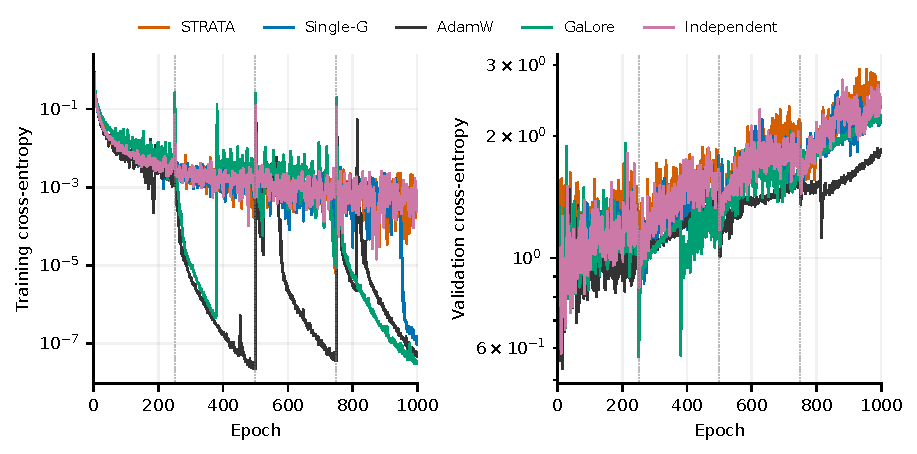
\includegraphics[width=.98\linewidth]{figures/fig_cifar10_shift_complete.pdf}
\caption{\textbf{Completed CIFAR-10 label-shift losses.} Raw training and validation cross-entropy for all five validation-selected configurations. Vertical guides mark phase boundaries at epochs 250, 500, and 750; the validation weighting changes across phases. Every trajectory finishes 1000 epochs. No smoothing or extrapolation.}\label{fig:cifar10-shift-complete}
\end{figure}
